
\begin{enumerate}[label=\thesection.\arabic*,ref=\thesection.\theenumi]
\item An arch is in the form of a parabola with its axis vertical. The arch is 10m high and 5m wide at the base. How wide is it 2m from the vertex of the parabola?
\label{chapters/11/11/5/2}
\iffalse

\documentclass[journal,10pt,twocolumn]{article}
\usepackage{graphicx}
\usepackage[margin=0.5in]{geometry}
\usepackage[cmex10]{amsmath}
\usepackage{array}
\usepackage{booktabs}
\usepackage{mathtools}
\usepackage{amssymb}
\title{\textbf{Conics Assignment}}
\author{lakshmi kamakshi}
\date{September 2022}
\providecommand{\norm}[1]{\left\lVert#1\right\rVert}
\providecommand{\abs}[1]{\left\vert#1\right\vert}
\let\vec\mathbf
\newcommand{\myvec}[1]{\ensuremath{\begin{pmatrix}#1\end{pmatrix}}}
\newcommand{\mydet}[1]{\ensuremath{\begin{vmatrix}#1\end{vmatrix}}}
\providecommand{\brak}[1]{\ensuremath{\left(#1\right)}}

\begin{document}

\maketitle
\paragraph{\textit{Problem Statement} -
\fi
\\
\solution
	\begin{figure}[!ht]
		\centering
 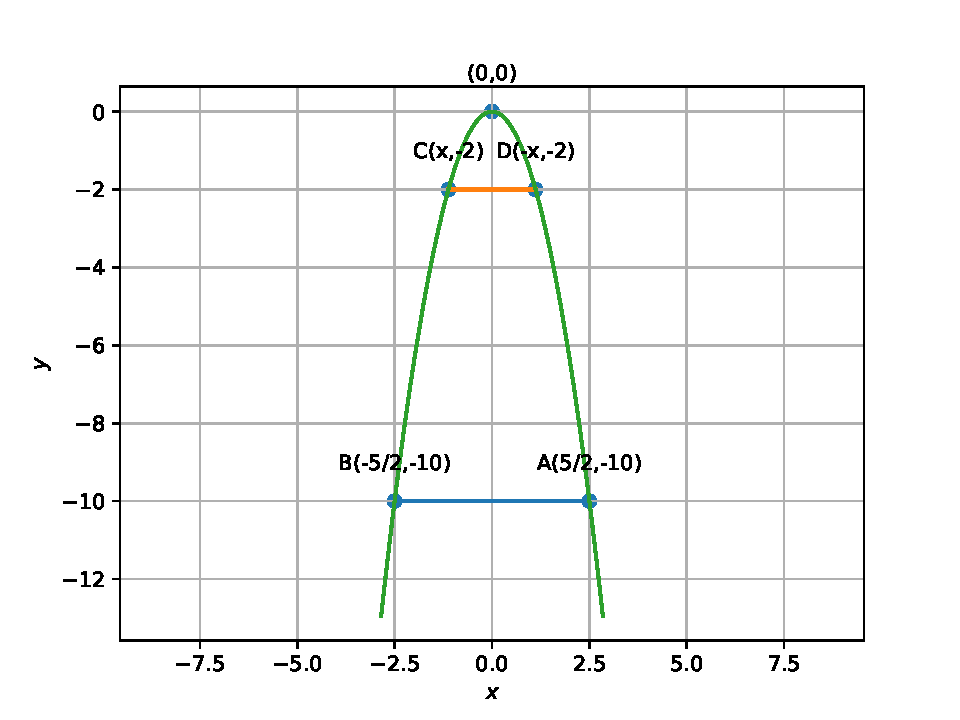
\includegraphics[width=\columnwidth]{chapters/11/11/5/2/figs/fig.pdf}
		\caption{}
		\label{fig:11/11/5/2}
  	\end{figure}
	\iffalse
} \vspace{5mm}

\section*{\large Solution}


Given, the axis of parabola is vertical,
\\ Let the equation of the axis be y-axis:
\begin{equation}
	\label{eq:parabola_q}
	\myvec{1\\0}\textbf{x}= 0
\end{equation}
\\ The above quadratic equation can be written in the general quadratic form as:

\begin{figure}[h]
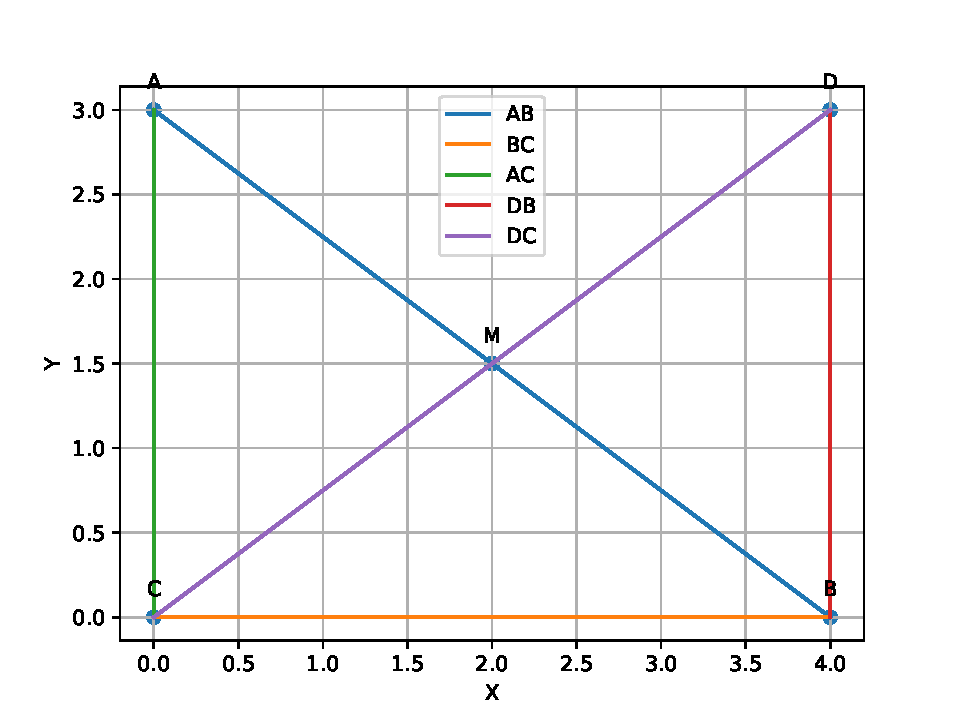
\includegraphics[width=0.8\columnwidth]{fig.pdf}
\end{figure}
\begin{equation}
	\label{eq:std_parabola}
	\textbf{x}^T\textbf{V}\textbf{x}+2\textbf{u}^T\textbf{x}+f=0
\end{equation}
where,
\begin{eqnarray}
\label{eq:Vec_V}
V = \myvec{1&0\\0&0}
\label{eq:Vec_U}
\\ u=\myvec{0\\2a}
\end{eqnarray}
\begin{equation}
\\ f =0
\end{equation}
Given arch is 10m high and 5m wide at the base. So the point $(\frac{5}{2},-10)$ lies on the parabola
\begin{equation}
	\myvec{X_1} = \myvec{\frac{5}{2}\\-10}
\end{equation}
\\ Substitute the point $X_1$ \\
\begin{eqnarray}
	\myvec{X_1}^T \myvec{V} \myvec{X_1} +2\myvec{u^T} \myvec{X_1} = 0
\\	a = \frac{5}{32}
\end{eqnarray}
\\Now , the matrix u will be,
\begin{equation}
	\myvec{u} = \myvec{0\\\frac{5}{16}}
\end{equation}
\\We need to find the width of parabola at a height of $2m$ from the vertex.So,the line parallel to x axis and passing through point $(0,-2)$ intersects the conic at 2 places C and D.
\\The line parallel to x-axis and passing through point $(0,-2)$ is
\begin{align}
	\myvec{X}\myvec{0\\1}^T = \myvec{2}
\end{align}
The points of intersection of the line 
\begin{align}
	L: \quad \vec{x} = \vec{q} + \mu \vec{m} \quad \mu \in \mathbf{R}
\label{eq:conic_tangent}
\end{align}
with the conic section  are given by
\begin{align}
\vec{x}_i = \vec{q} + \mu_i \vec{m}
\label{eq:conic_tangent_pts}
\end{align}
where 
{\tiny
\begin{multline}
\mu_i = \frac{1}
{
\vec{m}^T\vec{V}\vec{m}
}
\lbrak{-\vec{m}^T\brak{\vec{V}\vec{q}+\vec{u}}}
\\
\pm
\rbrak{\sqrt{
\sbrak{
\vec{m}^T\brak{\vec{V}\vec{q}+\vec{u}}
}^2
-
\brak
{
\vec{q}^T\vec{V}\vec{q} + 2\vec{u}^T\vec{q} +f
}
\brak{\vec{m}^T\vec{V}\vec{m}}
	}}
\label{eq:tangent_roots}
\end{multline}
}
\\
Substituting the line in the conic
\begin{align}
\brak{\vec{q} + \mu \vec{m}}^T\vec{V}\brak{\vec{q} + \mu \vec{m}}  
\\
+ 2 \vec{u}^T\brak{\vec{q} + \mu \vec{m}}+f &= 0
\\
\implies \mu^2\vec{m}^T\vec{V}\vec{m} + 2 \mu\vec{m}^T\brak{\vec{V}\vec{q}+\vec{u}} 
\\
+ \vec{q}^T\vec{V}\vec{q} + 2\vec{u}^T\vec{q} +f &= 0
\label{eq:conic_intercept}
\end{align}
Solving the above quadratic equations yeilds the roots.Let the point of intersections of line and curve be C and D.
\begin{align}
	C = q+ \mu_1m
	\\ D = q+ \mu_2m
\end{align}
\\The line CD will be
\begin{align}
	C-D = m(\mu_1-\mu_2)
	 \\ \textbf{m} = \myvec{1\\0}
\end{align}
The required width of parabola is the norm of the line CD.
\begin{align}
	||\boldsymbol{C-D}|| =
	2\sqrt{
\sbrak{
\vec{m}^T\brak{\vec{V}\vec{q}+\vec{u}}
}^2
-
\brak
{
\vec{q}^T\vec{V}\vec{q} + 2\vec{u}^T\vec{q} +f
}}
\end{align}
substitute the values of \vec{m},\vec{q},\vec{V} and \vec{u}
\begin{align}
	\frac{1}{2}||\vec{C-D}||^2 =
	\myvec{1&0}\brak{\vec{V}\myvec{0\\-2}+\vec{u}}\brak{\vec{V}\myvec{0\\-2}+\vec{u}}^T-
\end{align}
\begin{align*}
\brak
{
	\myvec{0&-2}\vec{V}\myvec{0\\-2} + 2\vec{u}^T\myvec{0\\-2} 
}
\end{align*}
 \begin{multiline}
	 \implies \sbrak{\myvec{1&0}\brak{\myvec{1&0\\0&0}\myvec{0\\-2} + \myvec{0\\\frac{5}{16}}}} \brak{\myvec{1&0\\0&0}\myvec{0\\-2} + \myvec{0\\\frac{5}{16}}}}^T  - \\
	 \\ \brak{\myvec{0&-2}\myvec{1&0\\0&0}\myvec{0\\-2} + 2\myvec{0 & \frac{5}{16}}\myvec{0\\-2} - 0} \\ \brak{\myvec{1&0}\myvec{1&0\\0&0}\myvec{1\\0}}
\end{multline}
\begin{align}
	\implies \sbrak{\myvec{1&0}\myvec{0\\\frac{5}{16}}}^2 - \brak{\myvec{0\\0}+2\myvec{0\\\frac{5}{-8}} - 0}(1) \\
 & = \myvec{5\\2}
\end{align}
\\The width of the Parabola at $2m$ height is the length of the line CD.  \begin{align} ||\vec{C-D}|| = \myvec{\sqrt{5}}$m$ \end{align} \section*{\large Construction} The input parameters are V,u,$X_1$,$y_2$ \\
\setlength\extrarowheight{7pt}
\begin{tabular}{|c|c|c|}
	\hline
	\textbf{Symbol}&\textbf{Value}&\textbf{Description}\\
	\hline
	$X_1$=\myvec{x_1\\y_1} & \myvec{\frac{5}{2}\\-10}&point at base \\[8pt]
	\hline
	$y_2$ & -2& height of point C\\[8pt]
	\hline
	$\vec{P}$&\myvec{0&1\\1&0}&eigenvectors of $\vec{V}$\\[8pt]
	\hline
	$\vec{c}$&$\myvec{0\\0}$&center of parabola\\
	\hline
	$\eta$&$\vec{u}^{\top}\vec{p}_1$&from Eq11\\[8pt]
	\hline
	$\lambda_2$&$\vec{e}_2^{\top}D\vec{e}_2$&from Eq9 \\[8pt]
	\hline
	$(\vec{A},\vec{B})$&\myvec{x_1&-x_1\\y_1&y_1}&points at the base\\[8pt]
	\hline
	$(\vec{C},\vec{D})$&\myvec{\sqrt{\frac{5y_2}{8}}&\sqrt{\frac{-5y_2}{8}}\\2&2}&points at 2m height\\[8pt]	\hline
\end{tabular}
\end{document}
\fi

\item 
    \item Find the area of the triangle formed by the lines joining the vertex 
    of the parabola 
    \begin{align}
        x^2 = 12y
        \label{eq:chapters/11/11/5/6/parabola}
    \end{align}
    to the ends of its latus rectum.
\label{chapters/11/11/5/6}
\iffalse
\documentclass[journal,12pt,twocolumn]{IEEEtran}
\usepackage{setspace}
\usepackage{gensymb}
\usepackage{xcolor}
\usepackage{caption}
\singlespacing
\usepackage{siunitx}
\usepackage[cmex10]{amsmath}
\usepackage{mathtools}
\usepackage{hyperref}
\usepackage{amsthm}
\usepackage{mathrsfs}
\usepackage{txfonts}
\usepackage{stfloats}
\usepackage{cite}
\usepackage{cases}
\usepackage{subfig}
\usepackage{longtable}
\usepackage{multirow}
\usepackage{enumitem}
\usepackage{bm}
\usepackage{mathtools}
\usepackage{listings}
\usepackage{tikz}
\usetikzlibrary{shapes,arrows,positioning}
\usepackage{circuitikz}
\renewcommand{\vec}[1]{\boldsymbol{\mathbf{#1}}}
\DeclareMathOperator*{\Res}{Res}
\renewcommand\thesection{\arabic{section}}
\renewcommand\thesubsection{\thesection.\arabic{subsection}}
\renewcommand\thesubsubsection{\thesubsection.\arabic{subsubsection}}

\renewcommand\thesectiondis{\arabic{section}}
\renewcommand\thesubsectiondis{\thesectiondis.\arabic{subsection}}
\renewcommand\thesubsubsectiondis{\thesubsectiondis.\arabic{subsubsection}}
\hyphenation{op-tical net-works semi-conduc-tor}

\lstset{
language=Python,
frame=single, 
breaklines=true,
columns=fullflexible
}
\begin{document}
\theoremstyle{definition}
\newtheorem{theorem}{Theorem}[section]
\newtheorem{problem}{Problem}
\newtheorem{proposition}{Proposition}[section]
\newtheorem{lemma}{Lemma}[section]
\newtheorem{corollary}[theorem]{Corollary}
\newtheorem{example}{Example}[section]
\newtheorem{definition}{Definition}[section]
\newcommand{\BEQA}{\begin{eqnarray}}
\newcommand{\EEQA}{\end{eqnarray}}
\newcommand{\define}{\stackrel{\triangle}{=}}
\newcommand{\myvec}[1]{\ensuremath{\begin{pmatrix}#1\end{pmatrix}}}
\newcommand{\mydet}[1]{\ensuremath{\begin{vmatrix}#1\end{vmatrix}}}
\bibliographystyle{IEEEtran}
\providecommand{\nCr}[2]{\,^{#1}C_{#2}} % nCr
\providecommand{\nPr}[2]{\,^{#1}P_{#2}} % nPr
\providecommand{\mbf}{\mathbf}
\providecommand{\pr}[1]{\ensuremath{\Pr\left(#1\right)}}
\providecommand{\qfunc}[1]{\ensuremath{Q\left(#1\right)}}
\providecommand{\sbrak}[1]{\ensuremath{{}\left[#1\right]}}
\providecommand{\lsbrak}[1]{\ensuremath{{}\left[#1\right.}}
\providecommand{\rsbrak}[1]{\ensuremath{{}\left.#1\right]}}
\providecommand{\brak}[1]{\ensuremath{\left(#1\right)}}
\providecommand{\lbrak}[1]{\ensuremath{\left(#1\right.}}
\providecommand{\rbrak}[1]{\ensuremath{\left.#1\right)}}
\providecommand{\cbrak}[1]{\ensuremath{\left\{#1\right\}}}
\providecommand{\lcbrak}[1]{\ensuremath{\left\{#1\right.}}
\providecommand{\rcbrak}[1]{\ensuremath{\left.#1\right\}}}
\theoremstyle{remark}
\newtheorem{rem}{Remark}
\newcommand{\sgn}{\mathop{\mathrm{sgn}}}
\newcommand{\rect}{\mathop{\mathrm{rect}}}
\newcommand{\sinc}{\mathop{\mathrm{sinc}}}
\providecommand{\abs}[1]{\left\vert#1\right\vert}
\providecommand{\res}[1]{\Res\displaylimits_{#1}} 
\providecommand{\norm}[1]{\lVert#1\rVert}
\providecommand{\mtx}[1]{\mathbf{#1}}
\providecommand{\mean}[1]{E\left[ #1 \right]}
\providecommand{\fourier}{\overset{\mathcal{F}}{ \rightleftharpoons}}
\providecommand{\ztrans}{\overset{\mathcal{Z}}{ \rightleftharpoons}}
\providecommand{\system}[1]{\overset{\mathcal{#1}}{ \longleftrightarrow}}
\newcommand{\solution}{\noindent \textbf{Solution: }}
\providecommand{\dec}[2]{\ensuremath{\overset{#1}{\underset{#2}{\gtrless}}}}
\let\StandardTheFigure\thefigure
\def\putbox#1#2#3{\makebox[0in][l]{\makebox[#1][l]{}\raisebox{\baselineskip}[0in][0in]{\raisebox{#2}[0in][0in]{#3}}}}
     \def\rightbox#1{\makebox[0in][r]{#1}}
     \def\centbox#1{\makebox[0in]{#1}}
     \def\topbox#1{\raisebox{-\baselineskip}[0in][0in]{#1}}
     \def\midbox#1{\raisebox{-0.5\baselineskip}[0in][0in]{#1}}

\vspace{3cm}
\title{Conic Assignment}
\author{Gautam Singh}
\maketitle
\bigskip

\begin{abstract}
    This document contains the solution to Question 6 of Exercise 5 in Chapter
    11 of the class 11 NCERT textbook.
\end{abstract}

\begin{enumerate}

    \solution 
    \fi

		Rewriting \eqref{eq:chapters/11/11/5/6/parabola} in matrix form,
    \begin{align}
        \vec{x}^\top\myvec{1&0\\0&0}\vec{x} + 2\myvec{0&-6}\vec{x} = 0
        \label{eq:chapters/11/11/5/6/parabola-mtx}
    \end{align}
    Since the parabola is clearly symmetric about the $y$-axis, we see that
    the directrix is parallel to the $x$-axis, thus
    \begin{align}
        \vec{n} = \myvec{0\\1}
        \label{eq:chapters/11/11/5/6/n}
    \end{align}
    Using the standard definition of the conic and equating $\vec{u}$ and $f$,
    \begin{align}
        \myvec{0\\-6} &= c\myvec{0\\1} - \vec{F} \label{eq:chapters/11/11/5/6/u-eqn} \\
        0 &= \norm{\vec{F}}^2 - c^2 \label{eq:chapters/11/11/5/6/f-eqn}
    \end{align}
    From \eqref{eq:chapters/11/11/5/6/u-eqn}, we have
    \begin{align}
        \vec{F} = \myvec{0\\c+6}
        \label{eq:chapters/11/11/5/6/F-c}
    \end{align}
    Using \eqref{eq:chapters/11/11/5/6/F-c} in \eqref{eq:chapters/11/11/5/6/f-eqn},
    \begin{align}
        \brak{c+6}^2&=c^2 \\
        \implies c&=-3
        \label{eq:chapters/11/11/5/6/c-sol}
    \end{align}
    Thus,
    \begin{align}
        \vec{F} = \myvec{0\\3}
    \end{align}
    The latus rectum of the parabola is the chord passing through the focus 
    parallel to the directrix. Its equation is given by
    \begin{align}
        \myvec{0&1}\vec{x} = \myvec{0&1}\myvec{0\\3} = 3
        \label{eq:chapters/11/11/5/6/latus-rectum}
    \end{align}
    Hence, for $\lambda \in \mathbb{R}$,
    \begin{align}
        \vec{x} = \lambda\myvec{1\\0} + \myvec{0\\3} = \myvec{\lambda\\3}
        \label{eq:chapters/11/11/5/6/x-general}
    \end{align}
    Adding \eqref{eq:chapters/11/11/5/6/parabola-mtx} to 12 times \eqref{eq:chapters/11/11/5/6/latus-rectum}, and
    using \eqref{eq:chapters/11/11/5/6/x-general}
    \begin{align}
        \vec{x}^\top\myvec{1&0\\0&0}\vec{x} &= 36 \\
        \implies \lambda^2 &= 36 \\
        \implies \lambda &= \pm 6
        \label{eq:chapters/11/11/5/6/x-latus}
    \end{align}
    Thus, the ends of the latus rectum are
    \begin{align}
        \vec{x} = \myvec{\pm 6\\3}
    \end{align}
    Since the vertex of the parabola is at $\vec{P} = \myvec{0\\0}$,
    we see that the area of the required triangle is
    \begin{align}
        \textrm{ar}\brak{\triangle PAB} = \frac{1}{2}\mydet{6&3\\-6&3} = 18\ \textrm{sq. units}
    \end{align}
    The situation is illustrated in Fig. \ref{fig:chapters/11/11/5/6/parabola}
    \begin{figure}[!ht]
        \centering
        %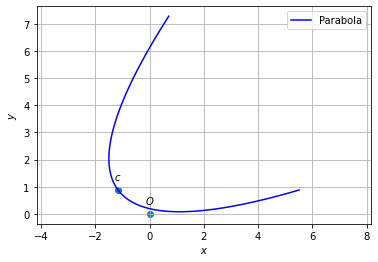
\includegraphics[width=\columnwidth]{chapters/11/11/5/6/figs/parabola.png}
        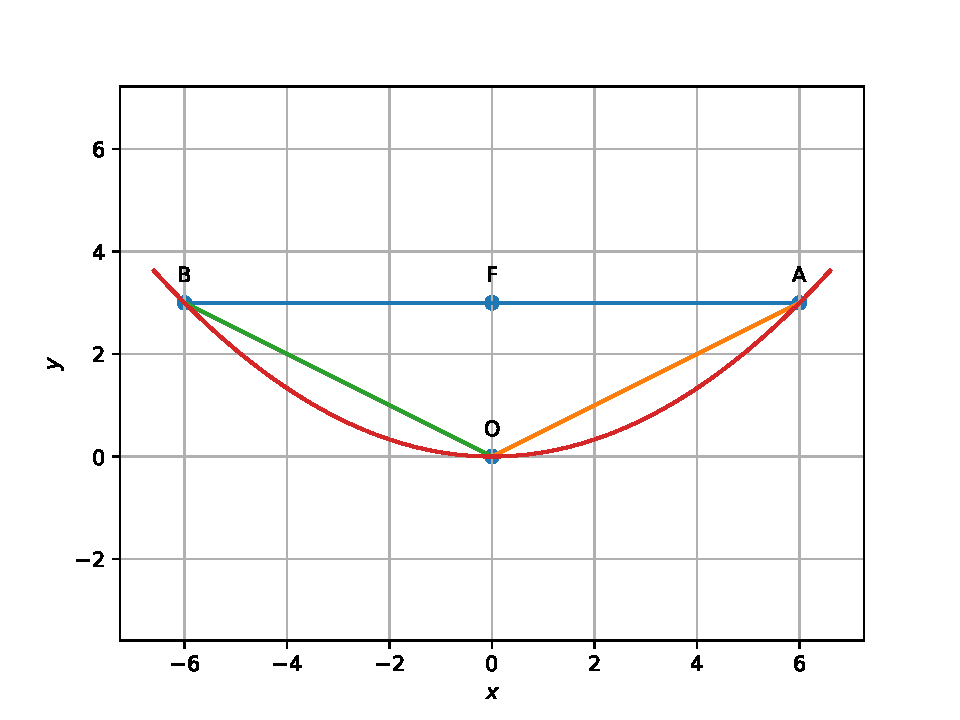
\includegraphics[width=\columnwidth]{chapters/11/11/5/6/figs/fig1.pdf}
        \caption{$PAB$ is the triangle whose area is to be found.}
        \label{fig:chapters/11/11/5/6/parabola}
    \end{figure}

\item An equilateral triangle is inscribed in the parabola $y^{2} = 4ax$,where one vertex is at the vertex of the parabola. Find the length of the side of the triangle.
\label{chapters/11/11/5/8}
\iffalse
\documentclass[journal,10pt,twocolumn]{article}
\usepackage{graphicx}
\usepackage[margin=0.5in]{geometry}
\usepackage[cmex10]{amsmath}
\usepackage{array}
\usepackage{booktabs}
\usepackage{mathtools}
\usepackage{amssymb}
\title{\textbf{Conics Assignment}}
\author{Alavala Chinnapa Reddy}
\date{September 2022}
\providecommand{\norm}[1]{\left\lVert#1\right\rVert}
\providecommand{\abs}[1]{\left\vert#1\right\vert}
\let\vec\mathbf
\newcommand{\myvec}[1]{\ensuremath{\begin{pmatrix}#1\end{pmatrix}}}
\newcommand{\mydet}[1]{\ensuremath{\begin{vmatrix}#1\end{vmatrix}}}
\providecommand{\brak}[1]{\ensuremath{\left(#1\right)}}
\providecommand{\lbrak}[1]{\ensuremath{\left(#1\right.}}
\providecommand{\rbrak}[1]{\ensuremath{\left.#1\right)}}
\providecommand{\sbrak}[1]{\ensuremath{{}\left[#1\right]}}
\begin{document}

\maketitle
\paragraph{\textit{Problem Statement} -
\fi
An equilateral triangle is inscribed in the parabola $y^{2} = 4ax$,where one vertex is at the vertex of the parabola. Find the length of the side of the triangle.
	\begin{figure}[!ht]
		\centering
 \includegraphics[width=\columnwidth]{chapters/11/11/5/8/figs/co.pdf}
		\caption{}
		\label{fig:11/11/5/8}
  	\end{figure}
\\
\solution
\iffalse
} \vspace{5mm}
\section*{\large Solution}


Given, the axis of parabola is horizotal.
\\ Given,one vertex of $\triangle$OAB is at vertex of parabola.

\begin{figure}[h]
\includegraphics[width=0.8\columnwidth]{figs/co.pdf}
\end{figure}
\begin{equation}
  \label{eq:std_parabola}
  \textbf{x}^T\textbf{V}\textbf{x}+2\textbf{u}^T\textbf{x}+f=0
\end{equation}
where,
\begin{eqnarray}
	\vec{O}=\myvec{0\\0}
\end{eqnarray}	
Equation Parabola is $y^2=4ax$\\
From $\triangle$OAB
\begin{eqnarray}
	\norm{\vec{A}}=\norm{\vec{B}}=\norm{\vec{A-B}}\\
	\norm{\vec{A}}^2=\norm{\vec{B}}^2=\norm{\vec{A-B}}^2\\
	\norm{\vec{A}}^2+\norm{\vec{B}}^2-2\vec{A}^T\vec{B}=\norm{\vec{A}}^2=\norm{\vec{B}}^2\\
	\frac{\vec{A}^T\vec{B}}{\norm{\vec{A}}^2}=\frac{\vec{A}^T\vec{B}}{\norm{\vec{B}^2}}=\frac{1}{2}
\end{eqnarray}
$\triangle$OAB is a equilateral triangle\\
$\alpha$=$60^{0}$\\
The side length of equilateral triangle,OA=OB=AB=r\\
Let
\begin{eqnarray}
	\vec{A}=\myvec{r\cos{\theta_1}\\r\sin{\theta_1}}\\
	\vec{B}=\myvec{r\cos{\theta_2}\\r\sin{\theta_2}}
\end{eqnarray}
\begin{eqnarray}
	\vec{A}^T\vec{B}=\frac{\norm{\vec{A}}^2}{2}\\
	r^2\cos{(\theta_1-\theta_2)}=\frac{r^2}{2}\\
	\theta_1-\theta_2=\cos{^{-1}\frac{1}{2}}
\end{eqnarray}
Given $\vec{A}$ satisfy the eq1
\begin{eqnarray}
	\vec{A}^T\vec{V}\vec{A}+2\vec{u}^T\vec{A}+f=0\\
	\vec{A}^T\vec{V}\vec{A}+2\vec{u}^T\vec{A}=0
\end{eqnarray}
\begin{equation}
	\myvec{r\cos{\theta_1}&r\sin{\theta_1}}\myvec{0&0\\0&1}\myvec{r\cos{\theta_1}\\r\sin{\theta_1}}+2\myvec{-2a&0}\myvec{r\cos{\theta_1}\\r\sin{\theta_1}}=0
\end{equation}
\begin{equation}
	\myvec{r\cos{\theta_1}&r\sin{\theta_1}}\myvec{0\\r\sin{\theta_1}}+2(-2ar\cos{\theta_1})=0
\end{equation}
\begin{eqnarray}
	r^2\sin{^2\theta_1}=4ar\cos{\theta_1}\\
	r=\frac{4a\cos{\theta_1}}{\sin{^2\theta_1}}
\end{eqnarray}
Similarly $\vec{B}$ satisfy the eq1
\begin{equation}
	r=\frac{4a\cos{\theta_2}}{\sin{^2\theta_2}}
\end{equation}
Form eq17 and eq18\\
Yeilding
\begin{eqnarray}
	\cos{(\theta_1+\theta_2)}=1\\
	\theta_1+\theta_2=\cos{^{-1}1}
\end{eqnarray}
Add eq11 and eq20\\
\begin{equation}
	\theta_1=\frac{\cos{^{-1}\frac{1}{2}+\cos{^{-1}1}}}{2}
\end{equation}
Subtract eq20 from eq11
\begin{equation}   
\theta_2=\frac{-\cos{^{-1}\frac{1}{2}+\cos{^{-1}1}}}{2}        
\end{equation}
 \section*{\large Construction} The input parameters are V,u,f \\
 $\vec{V}=\myvec{0&0\\0&1},\vec{u}=\myvec{-2a\\0},f=0$\\
\setlength\extrarowheight{7pt}
\begin{tabular}{|c|c|c|}
  \hline
  \textbf{Symbol}&\textbf{Value}&\textbf{Description}\\
  \hline
	a&1&\\
  \hline
	$\alpha$&$60^{0}$&$\angle{A}=\angle{B}=\angle{O}$\\
	\hline
	r&Solving eq18&OA=OB=AB\\
	\hline
  $\vec{O}$&$\myvec{0\\0}$&center of parabola and Point O\\
  \hline
	$\vec{A}$&$\myvec{r\cos{\theta_1}\\r\sin{\theta_1}}$&Point A\\[8pt]
  \hline
	$\vec{B}$&$\myvec{r\cos{\theta_2}\\r\sin{\theta_2}}$&Point B\\[8pt]  \hline
\end{tabular}
\end{document}
\fi

\end{enumerate}
In the each of the following Exercises, find the coordinates of the focus, axis of the parabola, the equation of the directrix and the length of the latus rectum.
\begin{enumerate}[label=\thesection.\arabic*,ref=\thesection.\theenumi,resume*]
\numberwithin{equation}{enumi}
\numberwithin{figure}{enumi}
\numberwithin{table}{enumi}

\item $y^2$=12x 
\label{chapters/11/11/2/1}
\\
\solution
\iffalse
\documentclass[12pt]{article}
\usepackage{graphicx}
\usepackage[none]{hyphenat}
\usepackage{graphicx}
\usepackage{listings}
\usepackage[english]{babel}
\usepackage{graphicx}
\usepackage{caption} 
\usepackage{booktabs}
\usepackage{array}
\usepackage{amssymb} % for \because
\usepackage{amsmath}   % for having text in math mode
\usepackage{extarrows} % for Row operations arrows
\usepackage{listings}
\lstset{
  frame=single,
  breaklines=true
}
\usepackage{hyperref}
  
%Following 2 lines were added to remove the blank page at the beginning
\usepackage{atbegshi}% http://ctan.org/pkg/atbegshi
\AtBeginDocument{\AtBeginShipoutNext{\AtBeginShipoutDiscard}}


%New macro definitions
\newcommand{\mydet}[1]{\ensuremath{\begin{vmatrix}#1\end{vmatrix}}}
\providecommand{\brak}[1]{\ensuremath{\left(#1\right)}}
\providecommand{\norm}[1]{\left\lVert#1\right\rVert}
\providecommand{\abs}[1]{\left\vert#1\right\vert}
\newcommand{\solution}{\noindent \textbf{Solution: }}
\newcommand{\myvec}[1]{\ensuremath{\begin{pmatrix}#1\end{pmatrix}}}
\let\vec\mathbf


\begin{document}

\begin{center}
\title{\textbf{Conic Sections - Parbola}}
\date{\vspace{-5ex}} %Not to print date automatically
\maketitle
\end{center}
\setcounter{page}{1}

\section{11$^{th}$ Maths - Chapter 11}
This is Problem-1 from Exercise 11.2
\begin{enumerate}
\solution 
\fi
The given equation of the parabola can be rearranged as
\begin{align}
    \label{eq:chapters/11/11/2/1/parabolaEq1}
    y^2-12x = 0
\end{align}
The above equation can be equated to the generic equation of conic sections
\begin{align}
	\label{eq:chapters/11/11/2/1/parabolaEq2}
	g\brak{\vec{x}} = \vec{x}^T\vec{V}\vec{x} + 2\vec{u}^T\vec{x} + f = 0 
\end{align}
Comparing coefficients of \eqref{eq:chapters/11/11/2/1/parabolaEq1} and \eqref{eq:chapters/11/11/2/1/parabolaEq2},
\begin{align}
	\label{eq:chapters/11/11/2/1/eqV}
	\vec{V} &= \myvec{ 0 & 0 \\ 0 & 1} \\
	\label{eq:chapters/11/11/2/1/eqU}
	\vec{u} &= -\myvec{6 \\ 0} \\
	\label{eq:chapters/11/11/2/1/eqF}
	f &= 0 
\end{align}
\begin{enumerate}
\item  
From \eqref{eq:chapters/11/11/2/1/eqV}, since $\vec{V}$ is already diagonalized, the Eigen values $\lambda_1$ and $\lambda_2$ are given as 
\begin{align}
	\label{eq:chapters/11/11/2/1/eqEigen1}
	\lambda_1 &= 0 \\
	\label{eq:chapters/11/11/2/1/eqEigen2}
	\lambda_2 &= 1 
\end{align}
and the eigenvector matrix
\begin{align}
	\vec{P} = \vec{I}.
\end{align}
\iffalse
The Eigen vector $\vec{p_1}$ corresponding to Eigen value $\lambda_1$ is computed as shown below
\begin{align}
	\vec{V} &= \myvec{ 0 & 0 \\ 0 & 1} \\
	\label{eq:chapters/11/11/2/1/eqLambda1}
	\vec{V}-\lambda_1\vec{I} &= \myvec{ 0 - \lambda_1 & 0 \\ 0 & 1-\lambda_1} 
\end{align}
Substituting value of $\lambda_1$ from \eqref{eq:chapters/11/11/2/1/eqEigen1} in \eqref{eq:chapters/11/11/2/1/eqLambda1}
\begin{align}
	\eqref{eq:chapters/11/11/2/1/eqLambda1} \implies  \myvec{  0 & 0 \\ 0 & 1}  \\
	\myvec{  0 & 0 \\ 0 & 1}\myvec{x_1 \\ x_2} &= \myvec{0 \\0} 
\end{align}
$x_1$ is free variable and $x_2 = 0$. \\
\fi
\begin{align}
	\therefore 
	%\vec{p_1} &= \myvec{1 \\ 0} \\
	\vec{n} &= \sqrt{\lambda_2}\vec{p_1} \\
%	&= \sqrt{1}\myvec{1 \\ 0} \\
	\label{eq:chapters/11/11/2/1/eqN}
	&= \myvec{1 \\ 0} 
\end{align}
Since
\begin{align}
	\label{eq:chapters/11/11/2/1/eqC}
	c = \frac{\norm{\vec{u}^2}-\lambda_2f}{2\vec{u}^\top\vec{n}},
\end{align}
Substituting values of $\vec{u}, \vec{n}, \lambda_2 \text{ and } f$ in \eqref{eq:chapters/11/11/2/1/eqC}
\begin{align}
	c &= \frac{6^2-1\brak{0}}{-2 \myvec{6 & 0}\myvec{1 \\ 0}} = -3 \\
\end{align}
The focus $\vec{F}$ of parabola is expressed as
\begin{align}
	\vec{F} &= \frac{ce^2\vec{n}-\vec{u}}{\lambda_2} \\
	&= \frac{-3\brak{1}^2\myvec{1 \\0} + \myvec{6 \\ 0}}{1} \\
	&= \myvec{3 \\ 0}
\end{align}
\item The directrix is given by
\begin{align}
	\vec{n}^\top\vec{x} &= c \\
	\label{eq:chapters/11/11/2/1/eqDir}
\implies	\myvec{1 & 0}\vec{x} &= -3
\end{align}

\item The equation for the axis of parabola passing through $\vec{F}$ and orthogonal to the directrix is given as  
\begin{align}
	\label{eq:chapters/11/11/2/1/eqAxis}
	\vec{m}^\top\brak{\vec{x}-\vec{F}} &= 0
\end{align}
where $\vec{m}$ is the normal vector to the axis and also the slope of the directrix.
\begin{align}
	\because \vec{n} = \myvec{1 \\ 0 }, \vec{m} &= \myvec{0 \\ 1} \\
	\eqref{eq:chapters/11/11/2/1/eqAxis} \implies \myvec{0 & 1}\myvec{\vec{x} - \myvec{3 \\ 0}} &= 0\\
	\text{or, }	\myvec{0 & 1}\vec{x} &= 0 
\end{align}
\item The latus rectum of a parabola is given by 
\begin{align}
	l &= \frac{\eta}{\lambda_2}  
	 = \frac{2\vec{u}^\top\vec{p_1}}{\lambda_2} \\
	 &= \frac{2\myvec{6 & 0}\myvec{1 \\ 0}}{1} \\
	 &= 12 \text{ units }
\end{align}
The relevant diagram is shown in Fig. \ref{fig:11/11/2/1Fig1}
\begin{figure}[!h]
	\begin{center}
		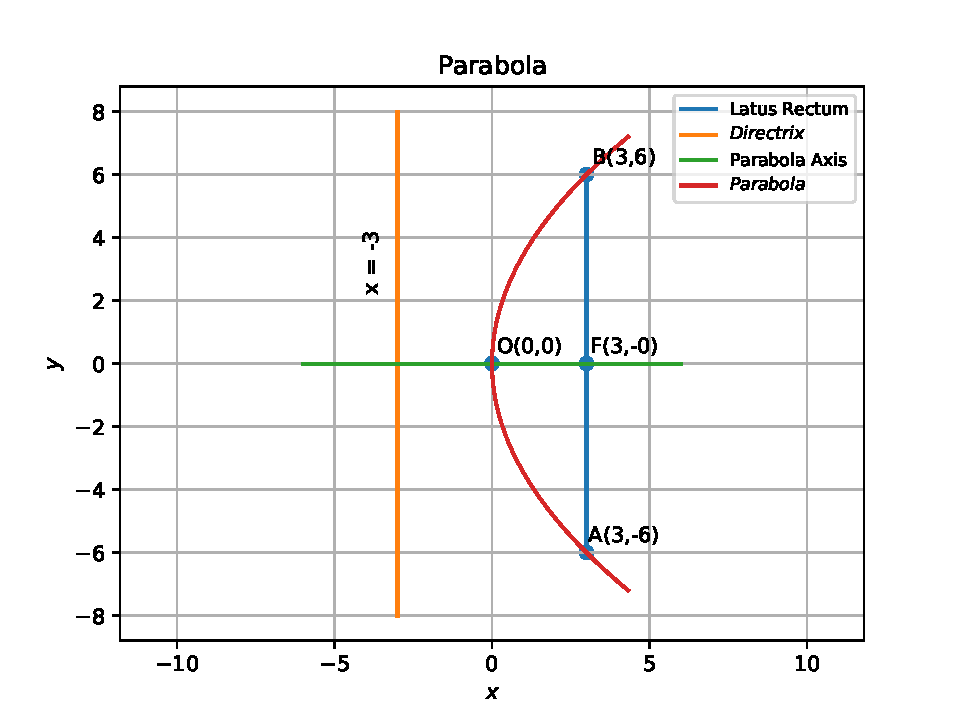
\includegraphics[width=\columnwidth]{chapters/11/11/2/1/figs/problem1.pdf}
	\end{center}
\caption{}
\label{fig:11/11/2/1Fig1}
\end{figure}
\end{enumerate}



\item $x^2$=6y 
\\
\solution
\iffalse
\documentclass[12pt]{article}
\usepackage{graphicx}
\usepackage{amsmath}
\usepackage{mathtools}
\usepackage{gensymb}

\newcommand{\mydet}[1]{\ensuremath{\begin{vmatrix}#1\end{vmatrix}}}
\providecommand{\brak}[1]{\ensuremath{\left(#1\right)}}
\providecommand{\norm}[1]{\left\lVert#1\right\rVert}
\newcommand{\solution}{\noindent \textbf{Solution: }}
\newcommand{\myvec}[1]{\ensuremath{\begin{pmatrix}#1\end{pmatrix}}}
\let\vec\mathbf

\begin{document}
\begin{center}
\textbf\large{CONIC SECTIONS}

\end{center}
\section*{Excercise 11.2}

Q2.Find the coordinates of the focus, axis of the parabola, the equation of the directrix and the length of the latus rectum of a parabola whose equation is given by $x^2=6y$.

\solution
\fi
The given equation of the parabola can be rearranged as
\begin{align}
	\label{eq:chapters/11/11/2/2/parabolaEq1}
	x^2-6y=0
\end{align}
The above equation can be equated to the generic equation of conic sections
\begin{align}
	\label{eq:chapters/11/11/2/2/parabolaEq2}
	g\brak{\vec{x}}=\vec{x}^\top \vec{V}\vec{x}+2\vec{u}^\top \vec{x}+f=0
\end{align}
Comparing the coefficients of both equations \eqref{eq:chapters/11/11/2/2/parabolaEq1} and \eqref{eq:chapters/11/11/2/2/parabolaEq2}
\begin{align}
	\label{eq:chapters/11/11/2/2/eqV}
	\vec{V} &= \myvec{1&0\\0&0}\\
	\label{eq:chapters/11/11/2/2/eqU}
	\vec{u} &= -\myvec{0\\3}\\
	\label{eq:chapters/11/11/2/2/eqF}
	f &= 0
\end{align}
\begin{enumerate}
\item From equation \eqref{eq:chapters/11/11/2/2/eqV}, since $\vec{V}$ is already diagonalized, the Eigen values $\lambda_1 \text{ and } \lambda_2$ are given as
\begin{align}
	\label{eq:chapters/11/11/2/2/eqEigen1}
	\lambda_1 &= 1\\
	\label{eq:chapters/11/11/2/2/eqEigen2}
	\lambda_2 &= 0
\end{align}
And the corresponding eigen vector matrix $\vec{P}$ is indentity, so the Eigen vector $\vec{p}_2$ corresponding to Eigen value $\lambda_2$ is
\begin{align}
	\vec{p}_2 &= \myvec{0\\1}\\
	\vec{n} &= \sqrt{\lambda_1}\vec{p}_2\\
		&= \sqrt{1}\myvec{0\\1}\\
		&= \myvec{0\\1}
\end{align}
Now,
\begin{align}
	\label{eq:chapters/11/11/2/2/eqC}
	c = \frac{\norm{\vec{u}}^2 - \lambda_1 f}{2\vec{u}^\top \vec{n}}
\end{align}
Substituting values of $\vec{u},\vec{n},\lambda_1 \text{ and } f$ in \eqref{eq:chapters/11/11/2/2/eqC}
\begin{align}
	c = \frac{3^2-1\brak{0}}{-2\myvec{0&3}\myvec{0\\1}} = -\frac{3}{2}
\end{align}
The focus $\vec{F}$ of parabola is expressed as
\begin{align}
	\vec{F} &= \frac{ce^2 \vec{n}-\vec{u}}{\lambda_1}\\
		&= \frac{-\frac{3}{2}\brak{1}^2 \myvec{0\\1}+\myvec{0\\3}}{1}\\
		&= \myvec{0\\\frac{3}{2}}
\end{align}
\item Equation of directrix is given as
\begin{align}
	\vec{n}^\top \vec{x} &= c\\
	\myvec{0&1}\vec{x} &= -\frac{3}{2}
\end{align}
\item The equation for the axis of parabola passing through $\vec{F}$ and orthogonal to the directrix is given as
\begin{align}
	\label{eq:chapters/11/11/2/2/eqM}
	\vec{m}^\top \brak{\vec{x}-\vec{F}} = 0
\end{align}
where $\vec{m}$ is the normal vector to the axis and also the slope of the directrix. Now since
\begin{align}
	\vec{n} = \myvec{0\\1}\\
	\vec{m} = \myvec{1\\0}
\end{align}
Substituting in \eqref{eq:chapters/11/11/2/2/eqM}
\begin{align}
	\myvec{1&0}\myvec{\vec{x}-\myvec{0\\\frac{3}{2}}}&=0\\
	\myvec{1&0}\vec{x} &= 0
\end{align}
\item The latus rectum of a parabola is given by
\begin{align}
	l&=\frac{\eta}{\lambda_1}\\
	 &=\frac{2\vec{u}^\top \vec{p}_2}{\lambda_1}\\
	 &=\frac{2\myvec{0&3}\myvec{0\\1}}{1}\\
	 &=6 \text{ units }
\end{align}
See Fig. \ref{fig:chapters/11/11/2/2/Fig1}
\begin{figure}[!h]
	\begin{center} 
	    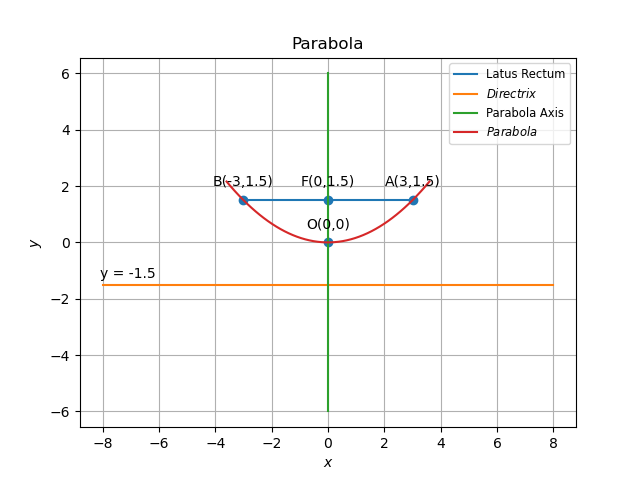
\includegraphics[width=\columnwidth]{chapters/11/11/2/2/figs/parabola}
	\end{center}
\caption{}
\label{fig:chapters/11/11/2/2/Fig1}
\end{figure}
\end{enumerate}





\item Find the coordinates of the focus, axis of the
parabola, the equation of the directrix and the length of the latus rectum of $y^2 = –8x$
\\
\solution
\iffalse
\documentclass[journal,12pt,twocolumn]{IEEEtran}
\usepackage{setspace}
\usepackage{gensymb}
\singlespacing
\usepackage[cmex10]{amsmath}
\usepackage{amsthm}
\usepackage{mathrsfs}
\usepackage{txfonts}
\usepackage{stfloats}
\usepackage{bm}
\usepackage{cite}
\usepackage{cases}
\usepackage{subfig}
\usepackage{longtable}
\usepackage{multirow}
\usepackage{enumitem}
\usepackage{mathtools}
\usepackage{steinmetz}
\usepackage{tikz}
\usepackage{circuitikz}
\usepackage{verbatim}
\usepackage{tfrupee}
\usepackage[breaklinks=true]{hyperref}
\usepackage{tkz-euclide}
\usetikzlibrary{calc,math}
\usepackage{listings}
    \usepackage{color}                                            %%
    \usepackage{array}                                            %%
    \usepackage{longtable}                                        %%
    \usepackage{calc}                                             %%
    \usepackage{multirow}                                         %%
    \usepackage{hhline}                                           %%
    \usepackage{ifthen}                                           %%
  %optionally (for landscape tables embedded in another document): %%
    \usepackage{lscape}     
\usepackage{multicol}
\usepackage{chngcntr}
\DeclareMathOperator*{\Res}{Res}
\renewcommand\thesection{\arabic{section}}
\renewcommand\thesubsection{\thesection.\arabic{subsection}}
\renewcommand\thesubsubsection{\thesubsection.\arabic{subsubsection}}

\renewcommand\thesectiondis{\arabic{section}}
\renewcommand\thesubsectiondis{\thesectiondis.\arabic{subsection}}
\renewcommand\thesubsubsectiondis{\thesubsectiondis.\arabic{subsubsection}}

% correct bad hyphenation here
\hyphenation{op-tical net-works semi-conduc-tor}
\def\inputGnumericTable{}                                 %%

\lstset{
frame=single, 
breaklines=true,
columns=fullflexible
}

\begin{document}


\newtheorem{theorem}{Theorem}[section]
\newtheorem{problem}{Problem}
\newtheorem{proposition}{Proposition}[section]
\newtheorem{lemma}{Lemma}[section]
\newtheorem{corollary}[theorem]{Corollary}
\newtheorem{example}{Example}[section]
\newtheorem{definition}[problem]{Definition}
\newcommand{\BEQA}{\begin{eqnarray}}
\newcommand{\EEQA}{\end{eqnarray}}
\newcommand{\define}{\stackrel{\triangle}{=}}

\bibliographystyle{IEEEtran}
\providecommand{\mbf}{\mathbf}
\providecommand{\pr}[1]{\ensuremath{\Pr\left(#1\right)}}
\providecommand{\qfunc}[1]{\ensuremath{Q\left(#1\right)}}
\providecommand{\sbrak}[1]{\ensuremath{{}\left[#1\right]}}
\providecommand{\lsbrak}[1]{\ensuremath{{}\left[#1\right.}}
\providecommand{\rsbrak}[1]{\ensuremath{{}\left.#1\right]}}
\providecommand{\brak}[1]{\ensuremath{\left(#1\right)}}
\providecommand{\lbrak}[1]{\ensuremath{\left(#1\right.}}
\providecommand{\rbrak}[1]{\ensuremath{\left.#1\right)}}
\providecommand{\cbrak}[1]{\ensuremath{\left\{#1\right\}}}
\providecommand{\lcbrak}[1]{\ensuremath{\left\{#1\right.}}
\providecommand{\rcbrak}[1]{\ensuremath{\left.#1\right\}}}
\theoremstyle{remark}
\newtheorem{rem}{Remark}
\newcommand{\sgn}{\mathop{\mathrm{sgn}}}
\providecommand{\abs}[1]{\left\vert#1\right\vert}
\providecommand{\res}[1]{\Res\displaylimits_{#1}} 
\providecommand{\norm}[1]{\left\lVert#1\right\rVert}
\providecommand{\mtx}[1]{\mathbf{#1}}
\providecommand{\mean}[1]{E\left[ #1 \right]}
\providecommand{\fourier}{\overset{\mathcal{F}}{ \rightleftharpoons}}
\providecommand{\system}{\overset{\mathcal{H}}{ \longleftrightarrow}}
\newcommand{\solution}{\noindent \textbf{Solution: }}
\newcommand{\cosec}{\,\text{cosec}\,}
\providecommand{\dec}[2]{\ensuremath{\overset{#1}{\underset{#2}{\gtrless}}}}
\newcommand{\myvec}[1]{\ensuremath{\begin{pmatrix}#1\end{pmatrix}}}
\newcommand{\mydet}[1]{\ensuremath{\begin{vmatrix}#1\end{vmatrix}}}
\numberwithin{equation}{subsection}
\makeatletter
\@addtoreset{figure}{problem}
\makeatother

\let\StandardTheFigure\thefigure
\let\vec\mathbf
\renewcommand{\thefigure}{\theproblem}



\def\putbox#1#2#3{\makebox[0in][l]{\makebox[#1][l]{}\raisebox{\baselineskip}[0in][0in]{\raisebox{#2}[0in][0in]{#3}}}}
     \def\rightbox#1{\makebox[0in][r]{#1}}
     \def\centbox#1{\makebox[0in]{#1}}
     \def\topbox#1{\raisebox{-\baselineskip}[0in][0in]{#1}}
     \def\midbox#1{\raisebox{-0.5\baselineskip}[0in][0in]{#1}}

\vspace{3cm}


\title{Assignment 1}
\author{Jaswanth Chowdary Madala}





% make the title area
\maketitle

\newpage

%\tableofcontents

\bigskip

\renewcommand{\thefigure}{\theenumi}
\renewcommand{\thetable}{\theenumi}


\begin{enumerate}

\textbf{Solution:}
\fi
The given equation of the parabola can be rearranged as
\begin{align}
y^2+8x = 0
\label{eq:chapters/11/11/2/3/1}
\end{align}
The above equation can be equated to the generic equation of conic sections
\begin{align}
\text{g}\brak{\vec{x}} = \vec{x}^T\vec{V}\vec{x} + 2\vec{u}^T\vec{x} + f = 0
\label{eq:chapters/11/11/2/3/2} 
\end{align}
Comparing coefficients of \eqref{eq:chapters/11/11/2/3/1} and \eqref{eq:chapters/11/11/2/3/2}, we get the parameters as given in Table \ref{tab:chapters/11/11/2/3/1}
\begin{table}[h]
\centering
%%%%%%%%%%%%%%%%%%%%%%%%%%%%%%%%%%%%%%%%%%%%%%%%%%%%%%%%%%%%%%%%%%%%%%
%%                                                                  %%
%%  This is a LaTeX2e table fragment exported from Gnumeric.        %%
%%                                                                  %%
%%%%%%%%%%%%%%%%%%%%%%%%%%%%%%%%%%%%%%%%%%%%%%%%%%%%%%%%%%%%%%%%%%%%%%

\begin{center}
\begin{tabular}{|c|c|}
\hline
\textbf{Parameter}& \textbf{Value}\\ \hline
$\vec{V}$		 &	$\myvec{0&0\\0&1}$\\ \hline
$\vec{u}$		 &	$\myvec{4\\0}$\\ \hline
$f$				 &  0 \\ \hline
\end{tabular}
\end{center}

\caption{}
\label{tab:chapters/11/11/2/3/1}
\end{table}
\begin{enumerate}
\item Focus: Since $\vec{V}$ is already diagonalized, the Eigen values $\lambda_1$ and $\lambda_2$ are given as 
\begin{align}
\lambda_1 = 0,\,
\lambda_2 = 1 
\end{align}
and the eigenvector matrix
\begin{align}
	\vec{P} = \vec{I} \implies 
\vec{p_1} &= \myvec{1 \\ 0} \\
	\text{and }\vec{n} &= \sqrt{\lambda_2}\vec{p_1} 
= \myvec{1 \\ 0} 
\end{align}
%
Since
\begin{align}
\label{eq:chapters/11/11/2/3/3}
c = \frac{\norm{\vec{u}^2}-\lambda_2f}{2\vec{u}^\top\vec{n}},
\end{align}
Substituting values of $\vec{u}, \vec{n}, \lambda_2 \text{ and } f$ in \eqref{eq:chapters/11/11/2/3/3}, we get
\begin{align}
c &= \frac{4^2-1\brak{0}}{2 \myvec{4 & 0}\myvec{1 \\ 0}} = 2
\end{align}
The focus $\vec{F}$ of parabola is expressed as
\begin{align}
\vec{F} &= \frac{ce^2\vec{n}-\vec{u}}{\lambda_2} 
= \myvec{-2 \\ 0}
\end{align}
\item Directrix: The directrix is given by
\begin{align}
\vec{n}^\top\vec{x} &= c \\
\implies	\myvec{1 & 0}\vec{x} &= 2
\end{align}
%
\item Axis: The equation for the axis of parabola, passing through $\vec{F}$ and orthogonal to the directrix is given as  
\begin{align}
\vec{m}^\top\brak{\vec{x}-\vec{F}} &= 0
\label{eq:chapters/11/11/2/3/4}
\end{align}
where $\vec{m}$ is the normal vector to the axis and also the slope of the directrix. Since
\begin{align}
	\vec{n} = \myvec{1 \\ 0 },\,
	\vec{m} &= \myvec{0 \\ 1} \\
\end{align}
the axis is given by
\begin{align}
\myvec{0 & 1}\myvec{\vec{x} - \myvec{-2 \\ 0}} &= 0\\
\implies \myvec{0 & 1}\vec{x} &= 0 
\end{align}
\item Latus rectum: The latus rectum of a parabola is given by 
\begin{align}
	l &= \frac{\eta}{\lambda_2}  
	 = \frac{2\vec{u}^\top\vec{p_1}}{\lambda_2} \\
	 &= 8 \text{ units }
\end{align}
\end{enumerate}
See Fig. 
\ref{fig:chapters/11/11/2/3/1}.
\begin{figure}[ht]
\centering
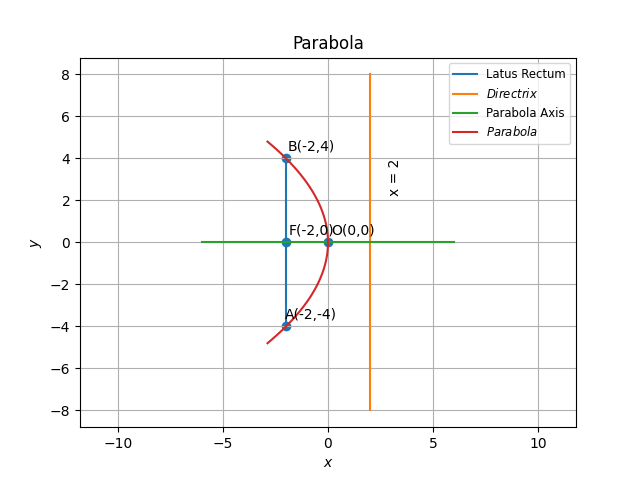
\includegraphics[width = \columnwidth]{chapters/11/11/2/3/figs/fig.png}
\caption{Graph}
\label{fig:chapters/11/11/2/3/1}
\end{figure}

\item $y^2$=-8x

\item $x^2$=-16y
\\
\solution
\iffalse
\documentclass[12pt]{article}
\usepackage{graphicx}
\usepackage{amsmath}
\usepackage{mathtools}
\usepackage{gensymb}

\newcommand{\mydet}[1]{\ensuremath{\begin{vmatrix}#1\end{vmatrix}}}
\providecommand{\brak}[1]{\ensuremath{\left(#1\right)}}
\providecommand{\norm}[1]{\left\lVert#1\right\rVert}
\newcommand{\solution}{\noindent \textbf{Solution: }}
\newcommand{\myvec}[1]{\ensuremath{\begin{pmatrix}#1\end{pmatrix}}}
\let\vec\mathbf

\begin{document}
\begin{center}
\textbf\large{CONIC SECTIONS}

\end{center}
\section*{Excercise 11.2.4}
	Find the coordinates of the focus, axis of the parabola, the equation of the directrix and the length of the latus rectum of a parabola whose equation is given by $x^2=-16y$.\\

\solution
\fi
The given equation of the parabola can be written as
\begin{align}
	\label{eq:chapters/11/11/2/4/parabolaEq1}
	x^2+16y=0
\end{align}
The general equation for conic section is
\begin{align}
	\label{eq:chapters/11/11/2/4/parabolaEq2}
	g\brak{\vec{x}}=\vec{x}^\top \vec{V}\vec{x}+2\vec{u}^\top \vec{x}+f=0
\end{align}
Comparaing both equations \eqref{eq:chapters/11/11/2/4/parabolaEq1} and \eqref{eq:chapters/11/11/2/4/parabolaEq2} we get,
\begin{align}
	\label{eq:chapters/11/11/2/4/eqV}
	\vec{V} &= \myvec{1&0\\0&0}\\
	\label{eq:chapters/11/11/2/4/eqU}
	\vec{u} &= \myvec{0\\8}\\
	\label{eq:chapters/11/11/2/4/eqF}
	f &= 0
\end{align}
\begin{enumerate}
\item As   $\vec{V}$ matrix is already diagonalized \eqref{eq:chapters/11/11/2/4/eqV}, the Eigen values $\lambda_1 \text{ and } \lambda_2$ are given as
\begin{align}
	\label{eq:chapters/11/11/2/4/eqEigen1}
	\lambda_1 &= 1\\
	\label{eq:chapters/11/11/2/4/eqEigen2}
	\lambda_2 &= 0
\end{align}
Eigen vector matrix $\vec{P}$ is identical the eigen vector $\vec{P}_2$ by eigen value $\lambda_2$ is 
\begin{align}
	\vec{p}_2 &= \myvec{0\\1}\\
	\vec{n} &= \sqrt{\lambda_1}\vec{p}_2\\
		&= \sqrt{1}\myvec{0\\1}\\
		&= \myvec{0\\1}
\end{align}
So,
\begin{align}
	\label{eq:chapters/11/11/2/4/eqC}
	 \frac{\norm{\vec{u}}^2 - \lambda_1 f}{2\vec{u}^\top \vec{n}}&= c
\end{align}
Substituting  $\vec{u},\vec{n},\lambda_1 \text{ and } f$ values in \eqref{eq:chapters/11/11/2/4/eqC} we get 
\begin{align}
	c = \frac{8^2-1\brak{0}}{2\myvec{0&8}\myvec{0\\1}} = 4
\end{align}
The focus $\vec{F}$ of parabola is 
\begin{align}
	\vec{F} &= \frac{ce^2 \vec{n}-\vec{u}}{\lambda_1}\\
		&= \frac{4\brak{1}^2 \myvec{0\\1}-\myvec{0\\8}}{1}\\
		&= \myvec{0\\-4}
\end{align}
\item Equation of directrix is given as
\begin{align}
	\vec{n}^\top \vec{x} &= c\\
	\myvec{0&1}\vec{x} &= 4\\
	\vec{x}&= 4
\end{align}
\item Equation for tha axis of parabola is 
\begin{align}
	\vec{m}^\top \brak{\vec{x}-\vec{F}} = 0\label{20}
\end{align}
where $\vec{m}$ is the normal vector to the axis and also the slope of the directrix
\begin{align}
	\vec{n} = \myvec{0\\1}\\
	\vec{m} = \myvec{1\\0}
\end{align}
Substituting in \eqref{20}
\begin{align}
	\myvec{1&0}\myvec{\vec{x}-\myvec{0\\-4}}&=0\\
	\myvec{1&0}\vec{x} &= 0\\
	\vec{x}=0
\end{align}
\item Latus rectum of  parabola is 
\begin{align}
	l&=\frac{\eta}{\lambda_1}\\
	 &=\frac{2\vec{u}^\top \vec{p}_2}{\lambda_1}\\
	 &=\frac{2\myvec{0&8}\myvec{0\\1}}{1}\\
	 &=16 \text{ units }
\end{align}
\begin{figure}[!h]
	\begin{center} 
	    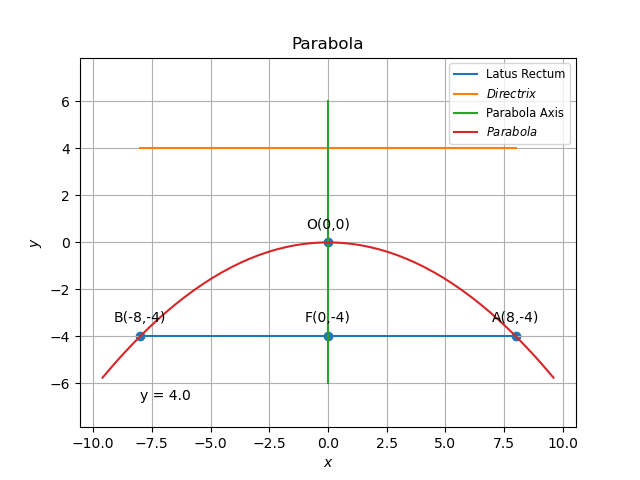
\includegraphics[width=\columnwidth]{chapters/11/11/2/4/figs/parabola}
	\end{center}
\caption{}
\label{fig:chapters/11/11/2/4/Fig1}
\end{figure}
\end{enumerate}


\item $y^2$=10x  

\item $x^2$=-9y  
\end{enumerate}

Each of the Exercises, find the equation of the parabola, that satisfies the given conditions.

\begin{enumerate}[label=\thesection.\arabic*,ref=\thesection.\theenumi,resume*]
\item Focus(6,0); directrix x=-6 
\item Focus(0,-3); directrix y=3
\item Vertex(0,0); Focus(3,0)
\item Vertex(0,0); Focus(-2,0) 
\item Vertex(0,0) passing through(2,3) and axis is along x-axis
\item Vertex(0,0) passing through(5,2) symmetric with respect to y-axis
\end{enumerate}
